
\section{Numerical Solution of Higher-Order Equations}
\label{sc:higher-order-numerics}

This section describes numerical methods for solving the higher-order equations discussed above. More specific details are given in Chapter \ref{ch:glissade}.

\subsection{Governing matrix equations}
We would like to solve the stress-balance equations \eqref{ho.eq.stress_balance_final_x} and \eqref{ho.eq.stress_balance_final_y} for the
horizontal velocity components $u$ and $v$.
 %\begin{align*}
% & x: \quad 4\frac{\partial }{\partial x}\left( \eta \frac{\partial u}{\partial x} \right)+\frac{\partial }{\partial y}\left( \eta \frac{\partial u}{\partial y} \right)+\frac{\partial }{\partial z}\left( \eta \frac{\partial u}{\partial z} \right) + \\
% & 2\frac{\partial }{\partial x}\left( \eta \frac{\partial v}{\partial y} \right)+\frac{\partial }{\partial y}\left( \eta \frac{\partial v}{\partial x} \right) = \rho g\frac{\partial s}{\partial x} \\ 
% & y: \quad 4\frac{\partial }{\partial y}\left( \eta \frac{\partial v}{\partial y} \right)+\frac{\partial }{\partial x}\left( \eta \frac{\partial v}{\partial x} \right)+\frac{\partial }{\partial z}\left( \eta \frac{\partial v}{\partial z} \right) + \\
% & 2\frac{\partial }{\partial y}\left( \eta \frac{\partial u}{\partial x} \right)+\frac{\partial }{\partial x}\left( \eta \frac{\partial u}{\partial y} \right) = \rho g\frac{\partial s}{\partial y} \\ 
%\end{align*}
%\begin{equation}
%  \begin{split}
%    & x: \quad 4\frac{\partial }{\partial x}\left( \eta \frac{\partial u}{\partial x} \right)+\frac{\partial }{\partial y}\left( \eta \frac{\partial u}{\partial y} \right)+\frac{\partial }{\partial z}\left( \eta \frac{\partial u}{\partial z} \right) + 2\frac{\partial }{\partial x}\left( \eta \frac{\partial v}{\partial y} \right)+\frac{\partial }{\partial y}\left( \eta \frac{\partial v}{\partial x} \right) = \rho g\frac{\partial s}{\partial x} \\ 
%    & y: \quad 4\frac{\partial }{\partial y}\left( \eta \frac{\partial v}{\partial y} \right)+\frac{\partial }{\partial x}\left( \eta \frac{\partial v}{\partial x} \right)+\frac{\partial }{\partial z}\left( \eta \frac{\partial v}{\partial z} \right) + 2\frac{\partial }{\partial y}\left( \eta \frac{\partial u}{\partial x} \right)+\frac{\partial }{\partial x}\left( \eta \frac{\partial u}{\partial y} \right) = \rho g\frac{\partial s}{\partial y} \\ 
%  \end{split}
%\end{equation}
%% SP: For Glissade, we don't do this (I don't think), so I'm commenting out this section for now.
%\subsection{Coordinate Transform}
%For ice sheet modeling, it is convenient to recast the governing equations using a dimensionless, stretched vertical coordinate (often called a sigma coordinates). The stretched vertical coordinate is defined as:
%
%\begin{align*}
%\sigma = \frac{(s - z)}{H}.
%\end{align*}
%
%This means that at the surface of the ice sheet $\sigma = 0$, and at the base $\sigma = 1$ regardless of the ice thickness.  As a result of this transformation, a coordinate ($x,y,z$) is mapped to ($x',y',\sigma$).  This means that function derivatives must be re-written (using $\frac{\partial f}{\partial x}$ as an example) as:
%
%\begin{align*}
%\frac{\partial f}{\partial x} = \frac{\partial f}{\partial x'} \frac{\partial x'}{\partial x} + \frac{\partial f}{\partial y'} \frac{\partial y'}{\partial x} + \frac{\partial f}{\partial \sigma} \frac{\partial \sigma}{\partial x}.
%\end{align*}
%
%Similarly for $\frac{\partial f}{\partial y}$ and $\frac{\partial f}{\partial z}$. We can simplify this by assuming that 
%
%\begin{align*}
%\frac{\partial x'}{\partial x}, \frac{\partial y'}{\partial y} = 1
%\end{align*}
%
%and
%
%\begin{align*}
%\frac{\partial x'}{\partial y}, \frac{\partial x'}{\partial z}, \frac{\partial y'}{\partial x}, \frac{\partial y'}{\partial z} = 0,
%\end{align*}
%
%which is valid if the bed and surface gradients are not too large. This simplifies the above to:
%
%\begin{align*}
%\frac{\partial f}{\partial x} = \frac{\partial f}{\partial x'} + \frac{\partial f}{\partial \sigma}\frac{\partial \sigma}{\partial x},
%\end{align*}
%
%\begin{align*}
%\frac{\partial f}{\partial y} = \frac{\partial f}{\partial y'} + \frac{\partial f}{\partial \sigma}\frac{\partial \sigma}{\partial y},
%\end{align*}
%
%\begin{align*}
%\frac{\partial f}{\partial z} = \frac{\partial f}{\partial \sigma}\frac{\partial \sigma}{\partial z}.
%\end{align*}
%
%Rescaling parameters $a_{x}$, $a_{y}$, $b_{x}$, $b_{y}$, and $c_{xy}$ are defined. For the $x$ derivative case (the $y$ derivative case is analogous) we have
%
%\begin{align*}
%a_{x} = \frac{1}{H}(\frac{\partial s}{\partial x'} - \sigma \frac{\partial H}{\partial x'}),
%\end{align*}
%
%\begin{align*}
%b_{x} = \frac{\partial a_x}{\partial x'} + a_x \frac{\partial a_x}{\partial \sigma} 
%    = \frac{1}{H} (\frac{\partial^2 s}{\partial x'^2} - \sigma \frac{\partial^2 H}{\partial x'^2} - 2a_x \frac{\partial H}{\partial x'}),
%\end{align*}
%
%\begin{align*}
%c_{xy} = \frac{\partial a_y}{\partial x'} + a_x \frac{\partial a_y}{\partial \sigma} 
%       = \frac{\partial a_x}{\partial y'} + a_y \frac{\partial a_x}{\partial \sigma}.
%\end{align*}
%
%Using these, expressions for the $x$ derivatives become:
%
%\begin{align*}
%\frac{\partial f}{\partial x} = \frac{\partial f}{\partial x'} + a_x \frac{\partial f}{\partial \sigma},
%\end{align*}
%
%\begin{align*}
% & \frac{\partial }{\partial x}\left( \eta \frac{\partial u}{\partial x} \right)=\frac{\partial }{\partial \hat{x}}\left( \eta \frac{\partial u}{\partial \hat{x}} \right)+\frac{\partial \sigma }{\partial \hat{x}}\frac{\partial }{\partial \sigma }\left( \eta \frac{\partial u}{\partial \hat{x}} \right)+\frac{\partial \sigma }{\partial \hat{x}}\frac{\partial }{\partial \hat{x}}\left( \eta \frac{\partial u}{\partial \sigma } \right)+ \\
%& \left( \frac{\partial \sigma }{\partial \hat{x}} \right)^{2}\frac{\partial }{\partial \sigma }\left( \eta \frac{\partial u}{\partial \sigma } \right)+\left( \frac{\partial _{{}}^{2}\sigma }{\partial \hat{x}_{{}}^{2}} \right)\eta \frac{\partial u}{\partial \sigma }
%\end{align*}
%
%where hatted values refer to the coordinate directions in sigma coordinates. Similarly, the first cross-stress term on the RHS is given by
%
%\begin{align*}
%&\frac{\partial }{\partial x}\left( \eta \frac{\partial v}{\partial y} \right)=\frac{\partial }{\partial \hat{x}}\left( \eta \frac{\partial v}{\partial \hat{y}} \right)\,+\frac{\partial \sigma }{\partial \hat{x}}\frac{\partial }{\partial \sigma }\left( \eta \frac{\partial v}{\partial \hat{y}} \right)\,+\frac{\partial \sigma }{\partial \hat{y}}\frac{\partial }{\partial \hat{x}}\left( \eta \frac{\partial v}{\partial \sigma } \right)\,+ \\
%&\frac{\partial \sigma }{\partial \hat{x}}\frac{\partial \sigma }{\partial \hat{y}}\frac{\partial }{\partial \sigma }\left( \eta \frac{\partial v}{\partial \sigma } \right)\,+\frac{\partial _{{}}^{2}\sigma }{\partial \hat{x}\partial \hat{y}}\eta \frac{\partial v}{\partial \sigma }\,
%\end{align*}
%
%
%One term has become five terms and each one of those is pretty ugly looking on its own. Luckily, there is a lot of symmetry here. Notice that if we wanted to design subroutines to discretize the terms on the RHS, we could re-use a lot of them by either applying them to the correct velocity component (to either the $u$ or the $v$ discretization) or by passing the appropriate arguments (by passing either the grid spacing in the $x$ direction or the $y$ direction, where appropriate).
%
%A similar transform is applied to each of the terms in the governing equations given above. At any point within the grid, the grid spacing, coordinate transform, and viscosity information associated with the unknown velocity components is made discrete using finite differences. This information ultimately equates to coefficients on the unknown velocities, allowing the governing equations over the entire grid (with appropriate discretizations for boundary conditions) to be recast as a system of $n$ equations in $n$ unknowns. In turn, this system is solved using standard linear algebraic methods for large, sparse systems of linear equations.
%% SP: For Glissade, we don't do this either, so commenting out this section for now. Note that I've copied some of it below in a new section, which gives a generic discussion of the matrix
%% form, to lead in to solution methods.
%\subsection{Operating Splitting}
%In the governing equations given above, note that for the \textit{x} equation we have moved all terms containing gradients in \textit{v} to the right-hand side (RHS) (and vice-versa for the \textit{y} equation). 
%
%This allows us to solve the equations using an $operator$ $splitting$ approach; for the $x$ equation, we treat $v$ as known (where we take the values of $v$ from the previous iteration, as discussed further below) and solve for $u$, and vice versa when we solve the $y$ equation for $v$. The splitting refers to the fact that we are breaking the multi-dimensional divergence operation into two steps; rather than solving one big matrix equation for $u$ and $v$ simultaneously, we solve two smaller matrix equations in sequence with one of the unknowns treated as a known source term on the RHS of the equation. This procedure was probably more common and important years ago when it was desirable to keep the matrix equations as small as possible for memory management issues. On today's machines, with fewer memory limitations (in particular when dealing with codes designed to run on parallel, distributed memory architectures) this splitting is not necessary and may even lead to some undesirable numerical side effects (i.e. a slow-down in the convergence of iterations used to treat nonlinearity in the governing equations).
%
%A general matrix form of the split equations, where coefficients on the $u$ and $v$ velocity components (i.e. viscosity, grid spacing, scalars) are contained in the block matrices \textbf{A}, is given by 
%
%\begin{align*}
%\begin{matrix}
%  \left[ \begin{matrix}
%   \mathbf{A}_{\mathbf{uu}} & \mathbf{0}  \\
%   \mathbf{0} & \mathbf{A}_{\mathbf{vv}}  \\
%\end{matrix} \right]\left[ \begin{matrix}
%   \mathbf{u}  \\
%   \mathbf{v}  \\
%\end{matrix} \right]=\left[ \begin{matrix}
%   \mathbf{b}_{\mathbf{u}}-\mathbf{A}_{\mathbf{uv}}\mathbf{v}  \\
%   \mathbf{b}_{\mathbf{v}}-\mathbf{A}_{\mathbf{vu}}\mathbf{u}  \\
%\end{matrix} \right] \\ 
%   \\ 
%  \mathbf{A}_{\mathbf{uu}}\mathbf{u}=\mathbf{b}_{\mathbf{u}}-\mathbf{A}_{\mathbf{uv}}\mathbf{v},\quad \quad \mathbf{A}_{\mathbf{vv}}\mathbf{v}=\mathbf{b}_{\mathbf{v}}-\mathbf{A}_{\mathbf{vu}}\mathbf{u} \\ 
%\end{matrix}
%\end{align*}
%
%where the \textbf{uu} subscript denotes block matrices containing coefficients for gradients on \textit{u} in the equation for the \textit{x} component of velocity (i.e. \textit{u}). The subscript \textbf{uv} denotes block matrices containing coefficients for gradients on \textit{v} in the equation for the \textit{x} component of velocity (and similarly for the \textbf{vv} and \textbf{vu} subscripts). On the right-hand side, the single subscripts \textbf{u} and \textbf{v} are attached to the geometric source terms for the \textit{x} and \textit{y} components of velocity, respectively.
\noindent
Any number of standard methods (e.g., finite differences, finite volumes, or finite elements) can be used to discretize these governing equations: i.e., to re-formulate them from their continuous, PDE form to a discontinuous, piecewise, algebraic approximation based on a specific computational mesh. 
In the limit, as the mesh spacing goes to zero, the difference between the solution to the actual PDE and its algebraic approximation also goes to zero. 
The Glissade dynamical core uses the Finite Element Method (FEM) to discretize the governing equations, as discussed in Chapter \ref{ch:glissade}. 
The result of the discretization is a set of linear algebraic equations that can be written in matrix form. 
An example is given below, where the coefficients of $u$ and $v$ are contained in block matrices \textbf{A}, given by 

\begin{equation}
  \begin{matrix}
    \left[ \begin{matrix}
        \mathbf{A}_{\mathbf{uu}} & \mathbf{A}_{\mathbf{uv}}  \\
        \mathbf{A}_{\mathbf{vu}} & \mathbf{A}_{\mathbf{vv}}  \\
      \end{matrix} \right]\left[ \begin{matrix}
        \mathbf{u}  \\
        \mathbf{v}  \\
      \end{matrix} \right]=\left[ \begin{matrix}
        \mathbf{b}_{\mathbf{u}}  \\
        \mathbf{b}_{\mathbf{v}}  \\
      \end{matrix} \right], \\ 
    \\ 
    \mathbf{A}_{\mathbf{uu}}\mathbf{u} + \mathbf{A}_{\mathbf{uv}}\mathbf{v} =\mathbf{b}_{\mathbf{u}},
    \quad \quad \mathbf{A}_{\mathbf{vu}}\mathbf{u} + \mathbf{A}_{\mathbf{vv}}\mathbf{v} =\mathbf{b}_{\mathbf{v}}. \\ 
  \end{matrix}
\end{equation}

\noindent
Here the \textbf{uu} subscript denotes block matrices containing coefficients for gradients of \textit{u} in the equation for the \textit{x} component of velocity (i.e., \textit{u}). The subscript \textbf{uv} denotes block matrices containing coefficients for gradients of \textit{v} in the equation for the \textit{x} component of velocity (and similarly for the \textbf{vu} and \textbf{vv} subscripts). On the right-hand side, the subscripts \textbf{u} and \textbf{v} are attached to the geometric source terms for the \textit{x} and \textit{y} components of velocity, respectively.

\subsection{Treating nonlinearity through a fixed-point iteration}
The nonlinearity of the equations---the fact that the matrix coefficients (in particular, the effective viscosity) depend
on the velocity (or more specifically, the velocity gradients)---is handled through a fixed-point iteration. 
A general fixed-point iteration for a vector of unknowns \textit{u} can be written as 

\begin{equation}
  u^{k} = \mathbf{B}\left( u^{k-1} \right),
\end{equation}

\noindent
where $k$ is the current iteration index and \textbf{B} is a matrix operation performed on the components of $u$ obtained at the previous iteration, $k-1$. The fixed point occurs when the values of $u$ at $k$ and $k-1$ are equal to within some given tolerance, at which point the iteration process is halted. %CISM has options for implementing both Picard and Newton-based fixed-point iterations. 
For a Picard iteration, which is used in Glissade, the matrix coefficients with a velocity dependence are simply based on the velocities from the previous iteration. In other words, velocities obtained during iteration $k-1$ are used to calculate the strain rates appearing in the expression for effective viscosity at iteration $k$.

%\subsection{Final Matrix Form}
Accounting for %both the operator splitting and 
the Picard iteration on the effective viscosity, the final form of the matrix equations solved by Glissade becomes 

%% SP: This is the split form - below is the more general (non-split) version
%\begin{align*}
%\begin{matrix}
%  \left[ \begin{matrix}
%   \mathbf{A}_{\mathbf{uu}}^{k-1} & \mathbf{0}  \\
%   \mathbf{0} & \mathbf{A}_{\mathbf{vv}}^{k-1}  \\
%\end{matrix} \right]\left[ \begin{matrix}
%   \mathbf{u}^{k}  \\
%   \mathbf{v}^{k}  \\
%\end{matrix} \right]=\left[ \begin{matrix}
%   \mathbf{b}_{\mathbf{u}}-\mathbf{A}_{\mathbf{uv}}^{k-1}\mathbf{v}^{k-1}  \\
%   \mathbf{b}_{\mathbf{v}}-\mathbf{A}_{\mathbf{vu}}^{k-1}\mathbf{u}^{k-1}  \\
%\end{matrix} \right] \\ 
%   \\ 
%  \mathbf{A}_{\mathbf{uu}}^{k-1}\mathbf{u}=\mathbf{b}_{\mathbf{u}}-\mathbf{A}_{\mathbf{uv}}^{k-1}\mathbf{v}^{k-1},\quad \quad \mathbf{A}_{\mathbf{vv}}^{k-1}\mathbf{v}=\mathbf{b}_{\mathbf{v}}-\mathbf{A}_{\mathbf{vu}}^{k-1}\mathbf{u}^{k-1} \\ 
%\end{matrix}
%\end{align*}

\begin{align*}
\begin{matrix}
  \left[ \begin{matrix}
   \mathbf{A}_{\mathbf{uu}}^{k-1} & \mathbf{A}_{\mathbf{uv}}^{k-1}  \\
   \mathbf{A}_{\mathbf{vu}}^{k-1} & \mathbf{A}_{\mathbf{vv}}^{k-1}  \\
\end{matrix} \right]\left[ \begin{matrix}
   \mathbf{u}^{k}  \\
   \mathbf{v}^{k}  \\
\end{matrix} \right]=\left[ \begin{matrix}
   \mathbf{b}_{\mathbf{u}}^{k}  \\
   \mathbf{b}_{\mathbf{v}}^{k}  \\
\end{matrix} \right], \\ 
   \\ 
  \mathbf{A}_{\mathbf{uu}}^{k-1}\mathbf{u}^{k} + \mathbf{A}_{\mathbf{uv}}^{k-1}\mathbf{v}^{k} =\mathbf{b}_{\mathbf{u}}^{k},
  \quad \quad \mathbf{A}_{\mathbf{vu}}^{k-1}\mathbf{u}^{k} + \mathbf{A}_{\mathbf{vv}}^{k-1}\mathbf{v}^{k} =\mathbf{b}_{\mathbf{v}}^{k}, \\ 
\end{matrix}
\end{align*}

\noindent
%where the index $k$ denotes values associated with the current non-linear iteration (in the case of velocities, these are the values being solved for and in the case of the geometric forcing terms, these are the values associated with the current time step) and the index $k-1$ denotes a ``lagged" value, taken from solution at the end of the previous non-linear iteration. 
These equations form a linear system; for the solution at any particular iteration $k$, 
the matrix coefficients that depend on the velocity components $u$ and $v$ are held frozen during the solution.
This linear system can be solved using a variety of methods. For large, sparse systems, the preconditioned conjugate gradient (PCG) method 
or some related method (e.g., preconditioned BiCG or GMRES) is generally the most efficient. 
(Glissade forms a symmetric positive-definite matrix, as required for the PCG method.
$\mathbf{A_{uu}}$ and $\mathbf{A_{vv}}$ are symmetric, and $\mathbf{A_{uv}} = \mathbf{A_{vu}^T}$.) 
In this case the linear system is solved not exactly, but to within some small tolerance of the true solution.

%% SP: commenting this out for now, since Newton is not currently an option (but leaving in as a possibility for use in later versions)

%\subsection{Newton-based Methods for Solutions of the Non-linear System}
%Without any operator splitting, the generic matrix form of the equations to be solved can be written as
%
%\begin{align*}
%\mathbf{A}(\mathbf{u})\mathbf{u}=\mathbf{b}.
%\end{align*}
%
%The linearized form of the equations to be solved using the Picard solution can be written as
%
%\begin{align*}
%\mathbf{u}^{k}=\mathbf{A}(\mathbf{u}^{k-1})^{-1}\mathbf{b}.
%\end{align*}
%
%The full nonlinear system to be solved can be written as
%
%\begin{align*}
%\mathbf{F}(\mathbf{u})=\mathbf{A}(\mathbf{u})\mathbf{u}-\mathbf{b}
%\end{align*}
%
%with the solution for the uknown vector \textit{u} given by 
%
%\begin{align*}
%\mathbf{F}(\mathbf{u})=0.
%\end{align*}
%
%A Newton-based solution for this system of equations, based on a first-order Taylor series expansion about the solution for \textit{u} at iteration \textit{k-1}, can be written as
%
%\begin{align*}
%\mathbf{F}(\mathbf{u}^{k})=\mathbf{F}(\mathbf{u}^{k-1})+\mathbf{F}(\mathbf{u}^{k-1})\delta \mathbf{u}^{k-1},
%\end{align*}
%
%where
%
%\begin{align*}
%\mathbf{F}(\mathbf{u}^{k-1})=\mathbf{J}^{k-1}
%\end{align*}
%
%is the system Jacobian with individual components give by
%
%\begin{align*}
%J_{ij}=\frac{\partial F_{i}(\mathbf{u}^{k-1})}{\partial u_{j}}
%\end{align*}
%
%and 
%
%\begin{align*}
%\delta \mathbf{u}^{k-1}=\mathbf{u}^{k}-\mathbf{u}^{k-1}
%\end{align*}
%
%is the Newton update to be solved for. One method for doing so is by solving 
%
%\begin{align*}
%\delta \mathbf{u}^{k-1}=-\left( \mathbf{J}^{k-1} \right)^{-1}\mathbf{F}(\mathbf{u}^{k-1}).
%\end{align*}
%
%The advantage of Newton-based methods is that, with a good initial guess for the solution, convergence rates are very often quadratic (e.g. the residual decreases quadratically, so that at iteration \textit{k} one has a residual of 0.1, at iteration \textit{k+1}, a residual of 0.01, and at iteration \textit{k+2} a residual of 0.0001), whereas Picard-based iterations are much slower to converge. A figure comparing rates of convergence for Picard versus Newton on a CISM tests case is shown below (Figure \ref{fig:jfnk}. The Newton method is based on the work of Lemieux et al. ($J.$ $Comput.$ $Phys.$, \textbf{230}, 2011), which is discussed further below.
%
%\begin{figure}
%  \begin{center}
%    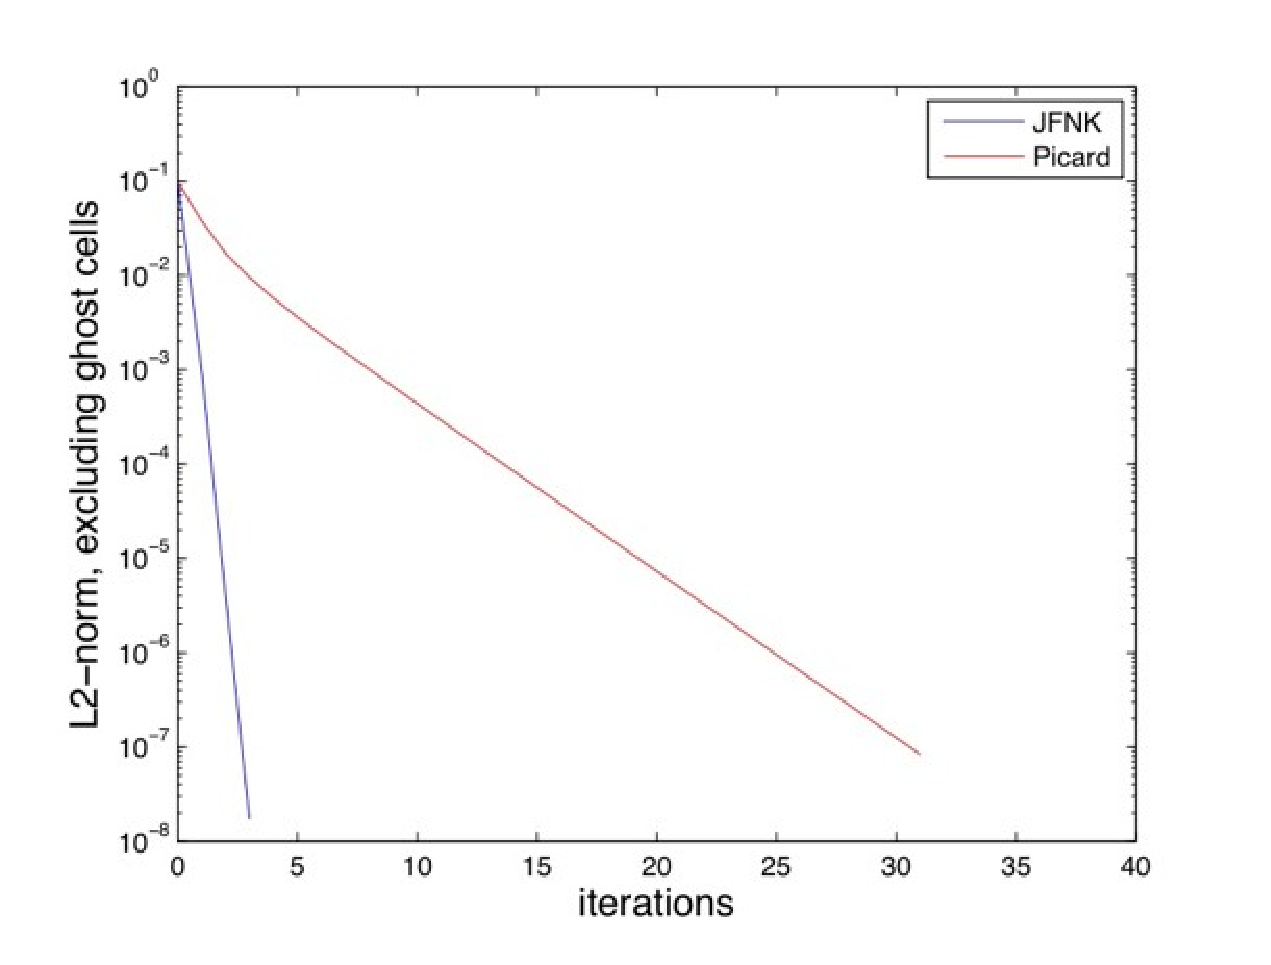
\includegraphics[width=0.9\columnwidth]{\dir/figs/Picard_vs_newton.eps}
%  \end{center}
%  \caption{Rates of convergence for the nonlinear iteration in CISM.}
%  \label{fig:jfnk}
%\end{figure} 
%
%\subsection{The Jacobian Free Approach}
%In practice, the model Jacobian may either be too difficult or to expensive too form. A Jacobian Free Newton-Krylov (JFNK) approach has recently been implemented in CISM (Leimieux et al., 2011), largely following methods discussed in Knoll and Keyes ($J.$ $Comput.$ $Phys.$, \textbf{193}, 2004).
%
%The crux of the method comes from noting that, when solving the last equation above using a Krylov method (e.g. Conjugate Gradients, GMRES, etc.) the solution for the Newton update is taken from a combination of Krylov vectors that span the subspace
%
%
%\begin{align*}
%span\left\{ \mathbf{r}_{0},\mathbf{Jr}_{0},\mathbf{J}^{2}\mathbf{r}_{0},...,\mathbf{J}^{n-1}\mathbf{r}_{0} \right\}=span\left\{ \mathbf{r}_{0},\mathbf{Jv}_{1},\mathbf{Jv}_{2},...,\mathbf{Jv}_{n-1} \right\}.
%\end{align*}
%
%This implies that, when using a Krylov method, one only ever needs to calculate matrix vector products of the form $\mathbf{Jv}$ when building up the subspace that approximates the solution vector $\delta \mathbf{u}$.
%
%Following Knoll and Keyes (2004), note that the necessary matrix vector products can be approximated through nonlinear function evaluations and a perturbation as
%
%\begin{align*}
%\mathbf{Jv}\approx \frac{\mathbf{F}\left( \mathbf{u}+\varepsilon \mathbf{v} \right)-\mathbf{F}\left( \mathbf{u} \right)}{\varepsilon }.
%\end{align*}
%
%It is not immediately obvious why this approximation is valid. To verify this, take a few steps back and consider a nonlinear system of equations of two variables, $u_{1}$ and $u_{2}$. The right-hand side of the above equation can be expanded as
%
%\begin{align*}
%\frac{\mathbf{F}\left( \mathbf{u}+\varepsilon \mathbf{v} \right)-\mathbf{F}\left( \mathbf{u} \right)}{\varepsilon }=\left[ \begin{matrix}
%   \frac{F_{1}\left( u_{1}+\varepsilon v_{1},u_{2}+\varepsilon v_{2} \right)-F_{1}(u_{1},u_{2})}{\varepsilon }  \\
%   \frac{F_{2}\left( u_{1}+\varepsilon v_{1},u_{2}+\varepsilon v_{2} \right)-F_{2}(u_{1},u_{2})}{\varepsilon }  \\
%\end{matrix} \right].
%\end{align*}
%
%A first-order Taylor series expansion approximation to this is given by
%
%\begin{align*}
%\frac{\mathbf{F}\left( \mathbf{u}+\varepsilon \mathbf{v} \right)-\mathbf{F}\left( \mathbf{u} \right)}{\varepsilon }\approx \left[ \begin{matrix}
%   \frac{F_{1}\left( u_{1},u_{2} \right)+\varepsilon v_{1}\frac{\partial F_{1}}{\partial u_{1}}+\varepsilon v_{2}\frac{\partial F_{1}}{\partial u_{2}}-F_{1}(u_{1},u_{2})}{\varepsilon }  \\
%   \frac{F_{2}\left( u_{1},u_{2} \right)+\varepsilon v_{1}\frac{\partial F_{2}}{\partial u_{1}}+\varepsilon v_{2}\frac{\partial F_{2}}{\partial u_{2}}-F_{2}(u_{1},u_{2})}{\varepsilon }  \\
%\end{matrix} \right],
%\end{align*}
%
%which collapses to
%
%\begin{align*}
%\frac{\mathbf{F}\left( \mathbf{u}+\varepsilon \mathbf{v} \right)-\mathbf{F}\left( \mathbf{u} \right)}{\varepsilon }\approx\left[ \begin{matrix}
%   v_{1}\frac{\partial F_{1}}{\partial u_{1}}+v_{2}\frac{\partial F_{1}}{\partial u_{2}}  \\
%   v_{1}\frac{\partial F_{2}}{\partial u_{1}}+v_{2}\frac{\partial F_{2}}{\partial u_{2}}  \\
%\end{matrix} \right].
%\end{align*}
%
%Finally, note that the right-hand side of the above equation is equal to 
%
%\begin{align*}
%\mathbf{Jv}\approx\left[ \begin{matrix}
%   v_{1}\frac{\partial F_{1}}{\partial u_{1}}+v_{2}\frac{\partial F_{1}}{\partial u_{2}}  \\
%   v_{1}\frac{\partial F_{2}}{\partial u_{1}}+v_{2}\frac{\partial F_{2}}{\partial u_{2}}  \\
%\end{matrix} \right],
%\end{align*}
%
%with the Jacobian matrix given by
%
%\begin{align*}
%\mathbf{J}=\left[ \begin{matrix}
%   \frac{\partial F_{1}}{\partial u_{1}} & \frac{\partial F_{1}}{\partial u_{2}}  \\
%   \frac{\partial F_{2}}{\partial u_{1}} & \frac{\partial F_{2}}{\partial u_{2}}  \\
%\end{matrix} \right].
%\end{align*}
%
%The matrix vector product \textbf{Jv} is what needs to be calculated repeatedly while building up the Krylov subspace vectors that combine to approximate the Newton update vector $\delta \mathbf{u}$.
%
%The important point is that at no point in this process does one need to calculate the entire Jacobian matrix. Another important point is that the accuracy of the approximation to the Jacobian is proportional to the small perturbation term, $\varepsilon$.

%\section{References}
%\begin{itemize}
%\item  {Knoll, D.A. and D.E. Keyes. Jacobian-free Newton-Krylov methods: a survey of approaches and applications, \textbf{193}, 357-397, 2004}.
%\end{itemize}
%
%\begin{itemize}
%\item  {Lemieux, J.F., S.F. Price, K.J. Evans, D. Knoll, A.G. Salinger, D. Holland, and A.J. Payne. Implementation of the Jacobian-Free Newton-Krylov method for solving the first-order ice sheet momentum balance, \textit{J. Comput. Phys.}, \textbf{230}, 6531-6545, doi:10.1016/j.jcp.2011.04.037, 2011}.
%\end{itemize}
%
%\end{document}
